\chapter{Architecture Constraints}

\section{Environment}
\label{sec:Environment}
\input{generated/tables/tools.tex}

\section{Layers Definition}

\begin{figure}[h]
	\centering
		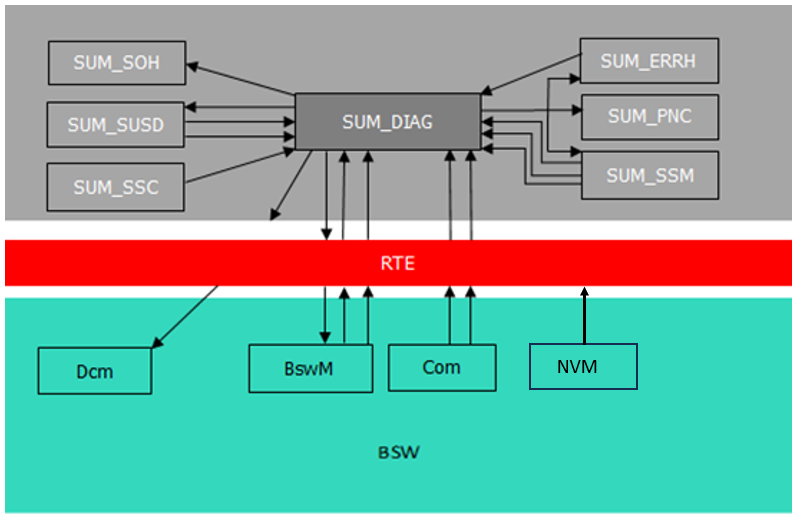
\includegraphics{images/layers}
	\caption{SUM_DIAG Layers}
\end{figure}

The applied system architecture is based on Autosar v4.0.3. For detailed information on it refer to Autosar.org website.

\section{Generic component interface}
\label{sec:Generic_component_interface}

\begin{figure}[h]
	\centering
		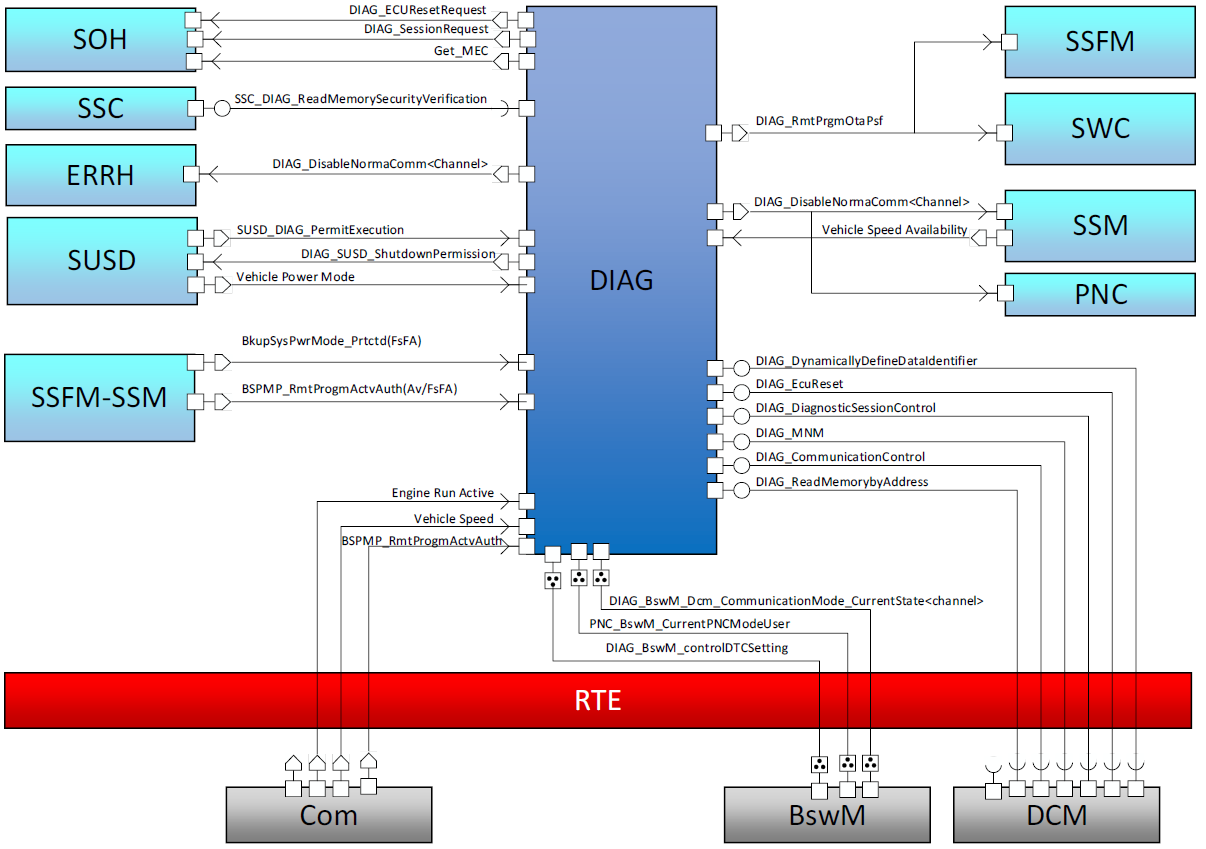
\includegraphics[width=15cm]{images/generic_component_interface}
	\caption{SUM_DIAG port interactions with the other modules}
\end{figure}

\Requirement{070}
{
}
{\Satisfies{SRS_DIAG 019} \Satisfies{SRS_DIAG 020} \Satisfies{SRS_DIAG 104} \Satisfies{SRS_DIAG 103} \Satisfies{SRS_DIAG 108}}
\input{generated/tables/port_interfaces.tex}

\section{Other constraints and assumptions}
\label{sec:Other_constraints}
\begin{itemize}
\item Runnable_DIAG_Main to be given high priority among runnables as it contains permit execution, which is needed for other functionalities in SUM DIAG.

\input{generated/tables/other_constraints.tex}

\item MEC Initial value is taken from the configured value of parameter “MecInitialValue” in DiagGeneral container.

\item The NvM block that contains the MEC must be added in the NvM configuration as a block that will be saved during the NvM shutdown and read upon power-on.

\item The NvM block that contains the OTA_PSF must be added in the NvM configuration as a block that will be saved during the NvM shutdown and read upon power-on.

\item The function Diag_SetProgConditions is used to write the InitialReflashFlag to NvM.

\Requirement{079}
{
\item The initialReflashFlag will be set to true upon a successful transition to the programming through the DIAG_SSC_InitialReflashFlag to be updated in NVM by SUM_SSC.
}
{\Satisfies{SRS_DIAG 105}}

\item Requirement [SUMDIAG_50] of ref. [1] is not fully implemented: as per GM clarification, SUM_DIAG receives only the vehicle power mode signal to derive Off_power_mode flag since its associated signal availability information is not provided by SUM_SUSD.
\end{itemize}
